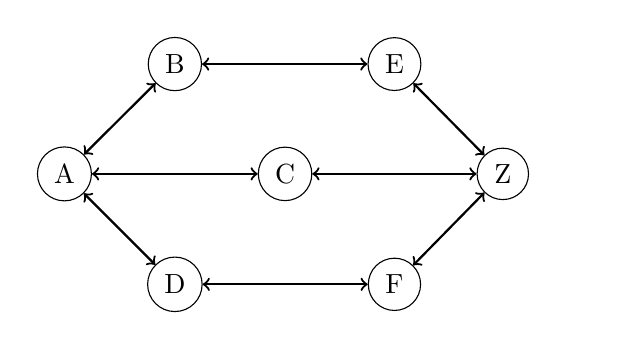
\begin{tikzpicture}
    \matrix[column sep=7mm, row sep=7mm]{
        & \node[draw, shape=circle](B){B}; & & 
        \node[draw, shape=circle](E){E}; & & \\
        \node[draw, shape=circle](A){A}; & & 
        \node[draw, shape=circle](C){C}; & & 
        \node[draw, shape=circle](Z){Z}; \\
        & \node[draw, shape=circle](D){D}; & & 
        \node[draw, shape=circle](F){F}; & & \\
    };
    \draw[<->, thick] (A) -- (C);
    \draw[<->, thick] (C) -- (Z);

    \draw[<->, thick] (A) -- (B);
    \draw[<->, thick] (B) -- (E);
    \draw[<->, thick] (E) -- (Z);

    \draw[<->, thick] (A) -- (D);
    \draw[<->, thick] (D) -- (F);
    \draw[<->, thick] (F) -- (Z);
\end{tikzpicture}